% Commented out: 
% \addbibresource
% \includepdf

\documentclass[12pt,letterpaper,english,bibliography=totocnumbered, abstract=on]{scrartcl}

\usepackage{indentfirst}
\usepackage[titletoc]{appendix}
%\usepackage[latin1]{inputenc}  % Enable direct input of special national characters
\usepackage[english]{babel}    % Language settings
\usepackage{lmodern}           % Enable Latin Modern fonts
\usepackage{color}
\usepackage{verbatim}
\usepackage[unicode=true,pdfusetitle,
bookmarks=true,bookmarksnumbered=false,bookmarksopen=false,
breaklinks=true,pdfborder={0 0 0},pdfborderstyle={},backref=false,colorlinks=true]
{hyperref}
\hypersetup{linkcolor=blue,citecolor=blue,urlcolor=blue}

\usepackage{booktabs}
\usepackage{multirow}
\usepackage{adjustbox}
\usepackage{threeparttable}
\usepackage[table]{xcolor}
\usepackage{csquotes}
\usepackage{soul} % for hiliting text: \hl

\usepackage[backend=biber, style=authoryear, maxbibnames=99, dashed=false]{biblatex}
\setlength\bibitemsep{2\itemsep}
\addbibresource{CASarticle.bib}
%\addbibresource{CRB.bib}

\usepackage{pdfpages}
\usepackage{float} % Allows use of H to place floats

\usepackage{pgfgantt}

\usepackage{framed}

\usepackage{array}

% Prevent page breaks within paragraphs
% https://tex.stackexchange.com/questions/21983/how-to-avoid-page-breaks-inside-paragraphs
\widowpenalties 1 10000


\usepackage{todonotes}

\begin{document}
	
\listoftodos



\title{Biological Control of the Cycad Aulacaspis Scale, \textit{Aulacaspis yasumatsui}}

\author{Contributions by Aubrey Moore}

\maketitle
%\footnote{\url{https://github.com/aubreymoore/2020-FS-CRB-biocontrol-project/blob/master/combined-proposal.pdf}}
\newpage
\tableofcontents

\pagebreak

\section{Abstract - Cave}

\section{Introduction - Cave}

\section{Economic impact of CAS - Cave and Wright}

\section{Ecological impact of CAS - Moore}

Ecological impact of CAS invasions varies greatly with location, largely due to differences in characteristics of host plant populations, climate, and presence of natural enemies. When CAS arrived in Florida (1995) and Hawaii (1998), it became an economic pest of ornamental cycads which could be protected using a combination of pesticide applications and biological control. However, when CAS arrived in Guam (2003), it started out as an economic pest of ornamental cycads \textit{Cycas revoluta} and \textit{Cycas micronesica} but rapidly spread to the wild \textit{Cycas micronesica} population, causing an uncontrolled island-wide outbreak. This chapter will be focused on the ecological impact to \textit{C. micronesica} and the forest ecosystem on Guam.

\subsection{\textit{C. micronesica} taxonomy and pre-invasion status} \textit{Cycas micronesica} was described as a species in 1994 \parencite{hillCycasRumphiiComplex1994}.
Prior to description, it was identified as \textit{C. rumphii} or \textit{C. circinalis}. 
This tree-sized cycad is endemic to Micronesia. It grows in the wild in a wide variety of habitats on Guam, the Northern Mariana Islands, the Yap Islands, and the Palau Islands.

Based on an island-wide census of Guam's trees performed by the U. S. Forest Service in in 2002, a year before arrival of CAS, \textit{C. micronesica} was identified as the most abundant tree in Guam's forests \cite{donnegon_guams_2004}. It thrived because it had evolved tolerance to local abiotic threats such as typhoons and drought and for this reason it was often used as a low maintenance ornamental plant. Indigenous people of the Mariana Islands, the Chamorros, used \textit{C. micronesica} as a source of starch. But there is no evidence that the plant was ever planted as a crop.   

\subsection{First detection and invasive pathway for arrival of \textit{A. yasumatsui} on Guam} 

Arrival of CAS on Guam was predicted: on February 13 2000 T. E. Marler published an article in the Gardening section of the Pacific Daily News entitled \textit{Looking out for scale insects} (\cite{haynesExoticInvasivePest2005}). Alarmed by establishment of CAS in Hawaii, Marler warned of pending arrival on Guam and pleaded for a ban cycad imports to the island. 

CAS was first detected in the Tumon Beach hotel area of Guam near the end of 2003 on \textit{C. micronesica} and \textit{C. revoluta} growing as ornamental plants at two hotels. In those days, almost every hotel on Guam had cycad displays near their entrances.

The invasion pathway along which CAS travelled to Guam is unknown.
It is likely that this pest arrived via importation of infested cycads from Hawaii, Florida or elsewhere. However, there are is no evidence of this: there are no records of legal cycad importation to Guam in the two years prior to detection of CAS on the island (R. Campbell, Guam Plant Inspection Facility, personal communication to AM).  

An intriguing alternative is that CAS arrived on Guam as crawlers. For several years prior to arrival, there was an active infestation of CAS on \textit{C. revoluta} growing in an outdoor garden at the Honolulu International Airport located within a few hundred meters of where passengers boarded a daily 7.5 hour flight to Guam. Possibly, crawlers were carried on clothing of passengers visiting this garden or airborne scale crawlers may have been blown into cargo holds, wheel wells, or other spaces on Guam-bound aircraft. The location of initial CAS detection sites in Tumon Bay are only about 1 km downwind of the Guam International Airport.

%Both of the leading actors in this story are relatively new to science: \textit{Aulacaspis yasumatsui} described as an herbivore of cycads in Thailand \parencite{takagiNewSpeciesAulacaspis1977} and \textit{Cycas micronesica} K. D. Hill 1994 was described as a cycad species endemic to Micronesia \parencite{hillCycasRumphiiComplex1994}.

\subsection{Impacts of CAS on the Guam population of \textit{C. micronesica}}

\begin{table}[p]
	\centering
	\label{tab:timeline}	
	\caption{Timeline for the Guam CAS infestation.}	
	\begin{tabular}{l>{\raggedright\arraybackslash}p{4.5in}}
		\hline
		2000 & T. E. Marler predicts of arrival of CAS on Guam in a Pacific Daily News article \parencite{haynesExoticInvasivePest2005} in response to detection of this pest in Florida during 1996 \parencite{howardAulacaspisYasumatsuiHemiptera1999a} and Hawaii during 1998 \parencite{heu2003sago}
		\\\hline
		2002 & An initial US Forest Service survey indicates that \textit{C. micronesica} is Guam's most abundant tree (with stem diameter greater than 5 inches) and estimates a population size of 1,571,556 \parencite{donnegon_guams_2004}
		\\\hline
		2003 & CAS first detected on ornamental \textit{Cycas revoluta} and \textit{C. micronesica} at hotels in Tumon Bay
		\\\hline
		2006 & \textit{C. micronesica} added to the IUCN Red List of Endangered and Threatened Species
		\\\hline
		2013 & A second US Forest Service survey ranks \textit{C. micronesica}, misidentified in the report as \textit{C. circinalis}, is Guam's xxrd most abundant tree (with stem diameter greater than 5 inches) and estimates a population size of n,nnn,nnn \parencite{lazaroGuamForestResources2020a}
		\\\hline
		2015 & \textit{C. micronesica} listed as a threatened species under the US Endangered Species Act \parencite{unitedstatesgovernmentEndangeredThreatenedWildlife2015}
		\\\hline
	\end{tabular}	
\end{table}

\begin{figure}[p]
	\centering
	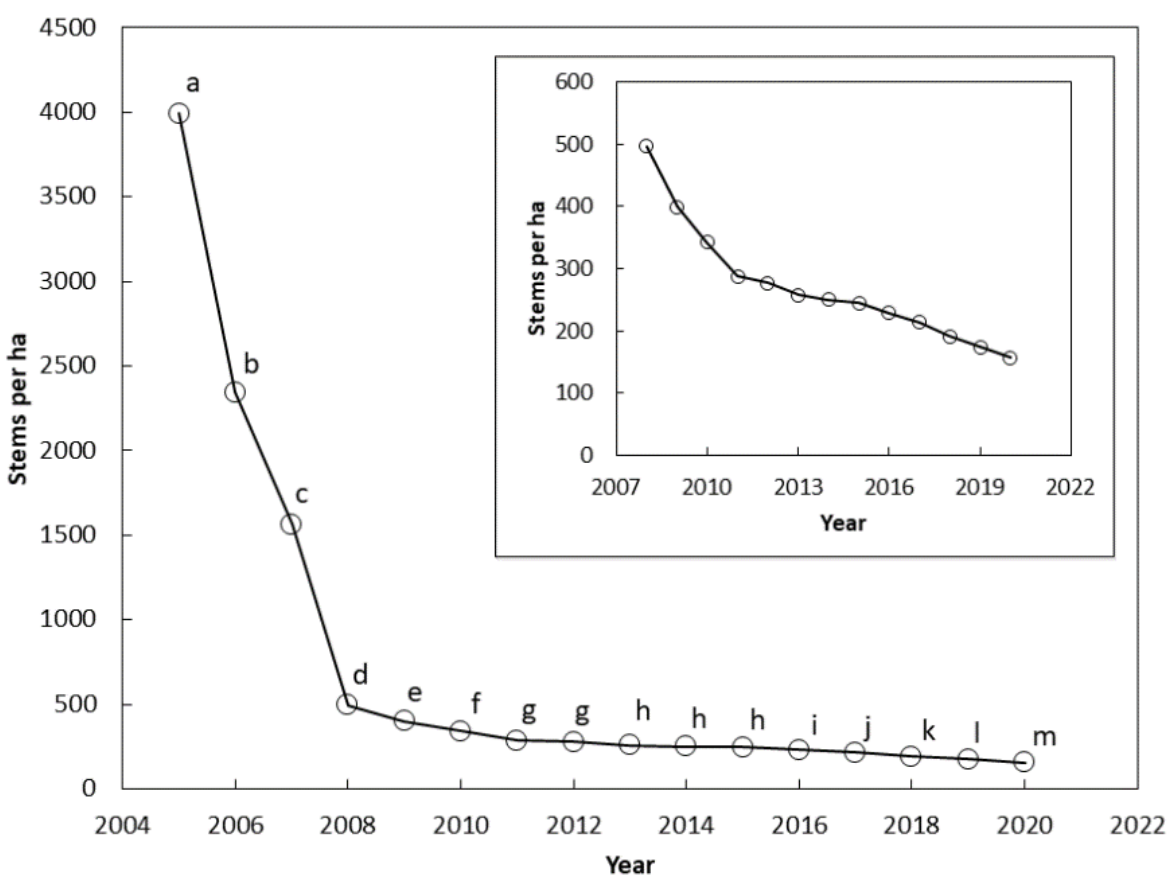
\includegraphics[width=\linewidth]{marler-stem-count}
	
	\caption{[From \cite{marlerLongitudeForestFragmentation2020}] The number
		of Cycas micronesica stems per ha (all size categories) among 12 Guam habitats
		from 2005 until 2020. The inset shows results from 2008 until 2020 with smaller vertical axis range. Ordinates of markers with the same letter are not significantly different.}
	
	\label{fig:marler-stem-count}
\end{figure}


The Guam CAS outbreak, which was severe and spread rapidly throughout the island (Table \ref{tab:timeline}, Figure \ref{fig:marler-stem-count}), was well documented by Marler and others. Within 12 years, \textit{C. micronesica} went from being the most abundant tree in Guam's forests to being listed under the U.S. Endangered Species Act. It should be noted that since arrival of CAS, several other recently arrived invasive insect species and even some native species have begun attacking and damaging Guam's cycads (
\cite{marlerPestsCycasMicronesica2006}, \cite{mooreCoalitionInvasiveSpecies2013}, \parencite{delosoBioticThreatsCycas2020a}). 
However, CAS is considered to be the prime driver of population decline because it is the only herbivore causing damage severe enough to result in mortality.

Rapid decline of the Guam \textit{C. micronesica} population was documented by 
\cite{marlerLongitudeForestFragmentation2020} (Figure \ref{fig:marler-stem-count}). Data are annual cycad stem counts in 120 permanent plots established after infestation of Guam's wild cycads, but prior to any mortality. It can be seen in the figure that cycad stem count declined to only 12.5\% of the original within the first 3 years of the survey (2005-2008) and continued to decline to only 4\% of the original count in succeeding years (2009-2020). In addition to high plant mortality surviving cycads stopped reproducing in the Guam plots: the last seedling (0-10 cm tall) was seen in 2006 and the last juvenile (10-100 cm tall) was seen in 2014. Between 2014 and 2020 the annual mortality rate for mature plants was relatively stable at about 14 per ha.

\todo{Mention forest survey results here?}

\subsection{Impacts of CAS on \textit{C. micronesica} individuals}

Immediate impacts of CAS on health of \textit{C. micronesica} individuals is very obvious. On Guam, unprotected plants typically die within 18 months (REF) after being infested. Several overlapping generations of CAS totally encrust all leaves within a few months of infestation. Plant mortality is caused by a combination of nutrient removal by CAS sap feeding plus blockage of photosynthesis. Scales covers of dead insects are tightly affixed to the plant and these do not easily wash off. So photosynthesis may be blocked even after scale insects are killed. \cite{muniappanCycadAulacaspisScale2012} suggest that toxic effects of CAS saliva may also be involved in cycad mortality. 

%Impacts to plants infested with CAS linger after the scale insects have been killed by insecticides or biocontrol agents. Scale covers block photosysnthesis \parencite{tangReportRecommendationsCycad2005a}.

Secondary impacts of CAS on health of C. micronesica individuals are not obvious.

\paragraph{Mature plants which have survived CAS infestation have reduced reproductive capacity}

Perhaps the most important secondary impact is much lower reproductive capability in plants recovering from CAS-infestation.  

\cite{marlerSourceSinkRelations2019} reported that seeds from CAS-infested plants are deficient in nonstructural carbohydrates  and germination rates are much lower: 43\% of seeds from healthy plants germinated versus 7\% of seeds from infested plants.

In addition, \cite{marlerAulacaspisYasumatsuiInvasion2021} reported that mature male plants which survived the initial CAS invasion have significantly smaller cones than prior to infestation. Average cone volume was 24\% of pre-infestation levels in 2007 and this increased to 57\% in 2021.

\paragraph{Mature plants which have survived CAS infestation are more susceptible to typhoon damage}  

\textit{C. micronesica} and other endemic plants on Guam have evolved tolerence for typhoon strength winds (greater than 118 km/h) because tropical cyclones frequently visit this island.
\parencite{marlerIncreasedThreatIsland2013} reported on results of sublethal winching stress tests performed on \textit{C. micronesica} stems to simulate effects of typhoon strength winds. Stems of plants which had not been infested by CAS were significantly stiffer than those which had been infested for either two or five years. Marler inferred from this finding that CAS-infested plants were much more susceptible to stem failure during typhoons.

Evidence for this hypothesis came from a damage survey after Typhoon Dolphin passed over Guam on May 15, 2015.
\cite{marler2016topographic} compare the level of damage from Typhoon Dolphin with that of a previous cyclone, Supertyphoon Paka:
\begin{displayquote}
Supertyphoon Paka caused severe damage to
Guam’s forest resources in 1997 when the C. micronesica population was
healthy and not threatened by any known invasive insect herbivores.
Less than 2\% of the healthy C. micronesica population exhibited
windsnap damage during peak winds of 298 km/h. In contrast,
Typhoon Dolphin’s peak winds of only 170 km/h. caused windsnap
of 6\% (mean of our eight sampling sites) of Guam’s unhealthy \textit{C.
micronesica} population after only 10 years of \textit{A. yasumatsui} infestations.
\end{displayquote}
Windsnap refers to stem failure. It is interesting to note that wind energy is a function of the square of wind speed. Therefor, maximum winds generated by Paka were about 3 times more powerfull than those of Dolphin.

\subsection{Cascading impacts of CAS on Guam's forest ecosystems}

Effects on soil \cite{marlerTwoCycadSpecies2020}

Symbiotic relationships

Gaps

\subsection{Prognosis for Guam's Forests} 

Pending extirpation of Guam's native cycads is not the first or last ecological disaster caused by invasive species in Guam's forests \parencite{moore_failed_2018}. The brown tree snake, \textit{Boiga irregularis}, first detected in 194? caused extinction or extirpation of all Guam's forest birds, also removing the ecosystem services they provided such as seed disperal, insectivory, and pollination. The coconut rhinoceros beetle, \textit{Oryctes rhinoceros}, first detected in 2007 is killing large numbers of coconut palms, \textit{Cocus nucifera}, and the introduced palma brava, \textit{Heterospathe elata}. These palm species were identified as Guam's second and third most abundant trees in the 2002 forestry survey \parencite{donnegon_guams_2004}.

\cite{haynesExoticInvasivePest2005}

\section{Natural enemies of CAS - Cave}

\section{Classical biological control}

\subsection{Florida - Cave}

\subsection{Hawaii - Wright}

\subsection{Guam - Moore}

\subsubsection{\textit{Rhyzobius lophanthae}}

About 100 adults of \textit{Rhyzobius lophanthae} were field collected on Maui and imported to Guam during November 2004. This coccinelid was originally 
introduced to California from Australia in 1892 and to Hawaii from California in 1894. It was observed feeding voraciously on CAS shortly after arrival of this new pest in Hawaii. 

\textit{R. lophanthae} was previously introduced to Guam on two separate occasions under various synonyms: \textit{R. satelles} Blackburn, \textit{Lindorus lophanthae} (Blaisdell), and \textit{R. pulchellus} Montrouzier (\cite{nafus_biological_1989}).
In 1925 and 1926 \textit{Rhyzobius satelles} was imported to Guam from California to control the coconut scale, \textit{Aspidiotus destructor} Signoret. However, attempts at field establishment failed.  

\cite{nafus_biological_1989} also reported:
\begin{displayquote}
 In 1971, \textit{Rhyzobius satelles} Blackburn (as \textit{R. pulchellus} Montrouzier) was introduced to Guam from New Caledonia to aid in the control of coconut scales and citrus scales. A single specimen of \textit{R. satelles} was recovered in 1978, indicating establishment. The beetle, however, is very uncommon; an intensive survey of coconut insects in 1984 yielded no specimens.
\end{displayquote}

The beetles from Maui were reared on scale-infested \textit{C. micronesica} cuttings placed in a large screened camping tent set up in a laboratory. Adult offspring were collected for field release by aspirating them from the walls of the tent into plastic vials. Field releases were initiated on February 16 2005 at the Guam National Wildlife Refuge at Ritidian Point. The beetles established readily. By July 7 2005 high densities on adults were observed on cycads anywhere within a 1 km radius of the release site.  Establishment and dispersion of the beetles were monitored using yellow sticky traps deployed between June 2005 and May 2006. Unexpectedly, we were also able to monitor CAS crawlers and adult males using these traps (Fig. \ref{fig:sticky-traps})  (\cite{moore_biological_2017-2}). Following establishment of \textit{R. lophanthae} at Ritidian Point, laboratory-reared and field-collected beetles were released at about 30 other sites throughout Guam. 

\begin{figure}[H]
	\centering
	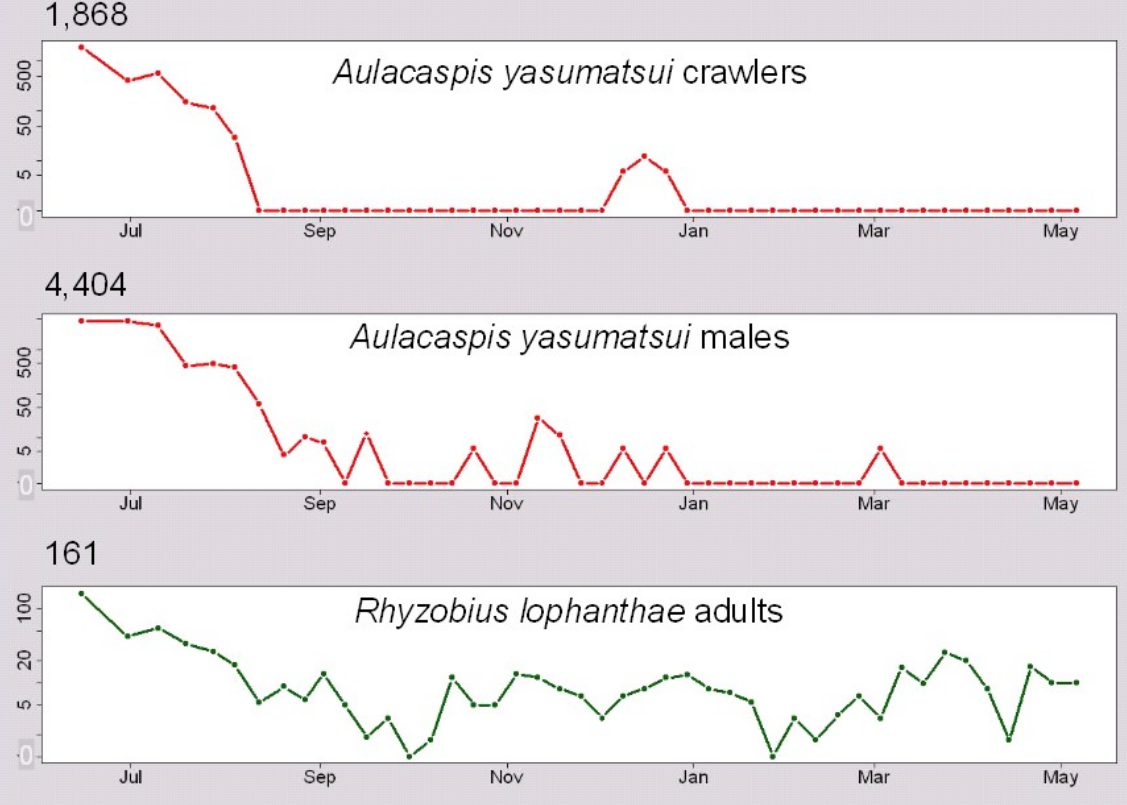
\includegraphics[width=\linewidth]{sticky-traps1}
	
	\caption{Insects trapped on yellow sticky cards at Ritidian Point, Guam following field release of Rhyzobius lophanthae in February, 2005. X axis runs from July 2005 through May 2006; Y-axis, in log scale, is number of insects trapped per square meter per day. [Figure from \cite{moore_biological_2013-2}]}
	
	\label{fig:sticky-traps}
\end{figure}

By about 2010, \textit{R. lophanthae} larvae or adults could be found on almost every CAS-infested cycad on Guam, preventing CAS from killing mature cycads. By 2010, about 90\% of wild cycads had been killed on Guam (REF). Unfortunately, the \textit{C. micronesica} population is not recovering because almost all seeds and seedlings are being killed by CAS and other causes (REF). \cite{marlerVerticalStratificationPredation2013} showed that \textit{R. lophanthae} predation of CAS is significantly reduced close to the ground and suggest that this may partially account for failure of the beetle to protect CAS seedlings. They also suggested:
\begin{displayquote}
The causes of reduced scale predation by
\textit{R. lophanthae} near the ground are unknown,
but a parasitoid biological control agent may
not exhibit these same limitations. Furthermore, because a parasitoid would be much
smaller than \textit{R. lophanthae}, it would likely be
better able to access scale infestations within
cracks and crevices on \textit{C. micronesica} and
\textit{C. revoluta} trees.
\end{displayquote}

\subsubsection{\textit{Coccobius fulvus}}  

\subsubsection{\textit{Aphytis lignanensis}}

\subsubsection{\textit{Arrhenophagus}}  

Ask Mark, Janis about Bernarr's report on fortuitous introduction of CAS parasitoids.

Ask Reddy about his report.

Ask Arnold Harra.


\subsection{Elsewhere - Cave}

\section{Prospects for future action - Cave, Wright, and Moore}

\newpage
\printbibliography[heading=bibintoc]

\end{document}
